% !TEX program = xelatex
% 编译：powershell -NoProfile -ExecutionPolicy Bypass -File scripts/build_latex.ps1 -Source paper/main.tex -OutputDirectory build/paper
\documentclass[withoutpreface,bwprint]{cumcmthesis}
\usepackage{cumcm2026}
\normalem
\usepackage{amsmath,amssymb,mathtools}
\usepackage{booktabs,longtable,tabularx,array,multirow}
\usepackage{graphicx,caption,float}
\usepackage{tikz}
\usetikzlibrary{arrows.meta,positioning}
\usepackage{enumitem}
\usepackage{fontspec}
\usepackage{fancyhdr}
\usepackage{xcolor}
\usepackage{hyperref}
\let\supercite\relax
\let\upcite\relax
\usepackage[backend=biber,style=gb7714-2015,sorting=none,url=false,doi=true]{biblatex}
\addbibresource{references.bib}
\setmainfont{Times New Roman}
\setCJKmainfont{SimSun}[BoldFont=SimHei,ItalicFont=KaiTi,BoldItalicFont=KaiTi]
\setCJKsansfont{SimHei}[BoldFont=SimHei]
\setCJKfamilyfont{zhsong}[BoldFont=SimHei,ItalicFont=KaiTi]{SimSun}
\setCJKfamilyfont{zhhei}[BoldFont=SimHei]{SimHei}
\renewcommand{\thesubsection}{\arabic{section}.\arabic{subsection}}
\renewcommand{\thesubsubsection}{\thesubsection.\arabic{subsubsection}}
\setlength{\parindent}{2em}
\setlength{\parskip}{0pt}
\renewcommand{\arraystretch}{1.17}
\hypersetup{unicode=true,colorlinks=true,linkcolor=black,citecolor=black,urlcolor=black}
\pagestyle{fancy}
\fancyhf{}
\fancyfoot[C]{\thepage}
\newtheorem{proposition}{命题}[section]
\renewcommand{\theproposition}{\arabic{section}.\arabic{proposition}}
\renewenvironment{proof}{\par\noindent\textbf{证明. }\ignorespaces}{\unskip\hfill$\square$\par}
\newcommand{\ind}{\mathbb{I}}
\newcommand{\E}{\mathbb{E}}
\newcommand{\Var}{\operatorname{Var}}
\newcommand{\Cov}{\operatorname{Cov}}
\newcommand{\AIV}{\mathrm{AIV}}
\newcommand{\HOT}{\mathrm{HOT}}
\newcommand{\CTQ}{\mathrm{CTQ}}
\newcommand{\DHI}{\mathrm{DHI}}
\newcommand{\MAB}{\mathrm{MAB}}
\newcommand{\ABL}{\mathrm{ABL}}
% Aggregates and figures from results/final-analysis/summary.json
% Source manifest SHA256: 7e885ceecf12a180349369ed9ddfc962ad71f1ea270f68b037a86a396430631d
% Summary SHA256: a181f0840a47c129aeb148f1ea5b36c5941a0943cd5fb1ebfa2acd8bfc28a64c
\newcommand{\FinalAbstractResults}{%
对 3515 个真实学生回合的分析得到任务候选 1010 条、贡献候选 776 条，同回合双维共同非空仅 48 条。秋、春任务候选高阶比例为 19.52\% 与 8.02\%，但把未知回合纳入有界情景后，学期差的符号无法确定。同一 352 回合上，双快严格候选经强复核由 110 条变为 86 条；复核同时产生新候选和撤回候选。356 个有任务候选的学生—学期单元均缺有效 CTQ；完整 AIV 无点分，保守范围揭示了补充过程证据的必要性。
}

\newcommand{\FinalSelectionResults}{%
为量化可判定性对学期比较的影响，固定候选标签，让其余回合的潜在层级在 L1 至 L6 间任取。令总回合为 $N$、候选数为 $n$、候选层级和为 $s$、候选高阶数为 $h$，得到
\begin{equation}\label{eq:unknown}
\mathrm{ABL}_{\rm raw}\in[(s+N-n)/N,(s+6(N-n))/N],\quad
\HOT\in[h/N,(h+N-n)/N].
\end{equation}
这是一种保留候选的条件构造，检查未知部分需要何种约束才能支持总体比较。
\begin{figure}[htbp]\centering
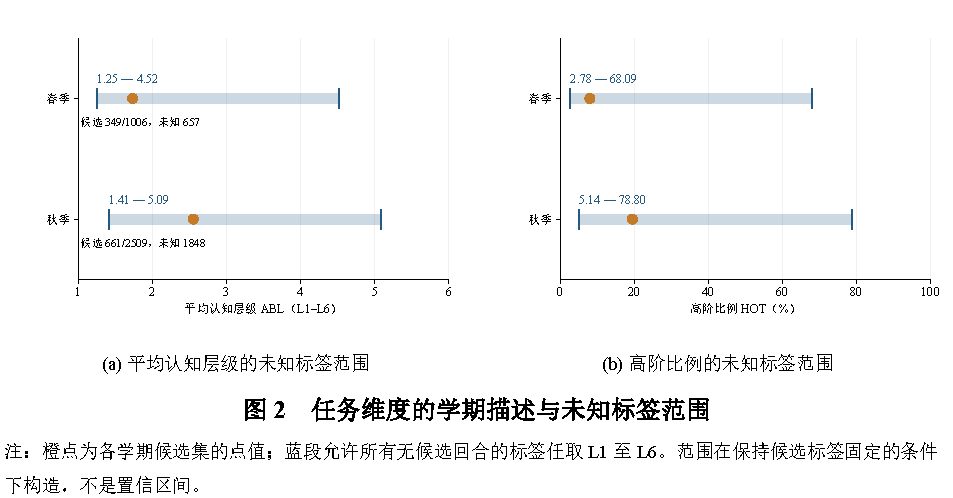
\includegraphics[width=\linewidth,height=.33\textheight,keepaspectratio]{../results/final-analysis/fig03_unknown_labels.pdf}
\caption{任务维度的学期描述与未知标签范围。橙点为各学期候选集；蓝段允许所有无候选回合取 L1 至 L6，范围为条件情景。}\label{fig:unknown}
\end{figure}
秋、春候选任务的平均层级分别为 2.554 与 1.734，高阶占比分别为 19.52\% 与 8.02\%；候选春减秋为 $-11.49$ 个百分点。扩展到全部合格回合后，两学期 HOT 分别在 $[5.14\%,78.80\%]$ 与 $[2.78\%,68.09\%]$ 内，春减秋范围为 $[-76.01,62.95]$ 个百分点。范围覆盖正、负方向，说明已知候选的学期差尚不足以确定总体过程差的方向。贡献维度的春减秋范围同样跨零（$[-80.74,79.10]$ 个百分点），因此后续 B 对两学期保留分层描述。
}

\newcommand{\FinalWorkflowResults}{%
\begin{figure}[htbp]\centering
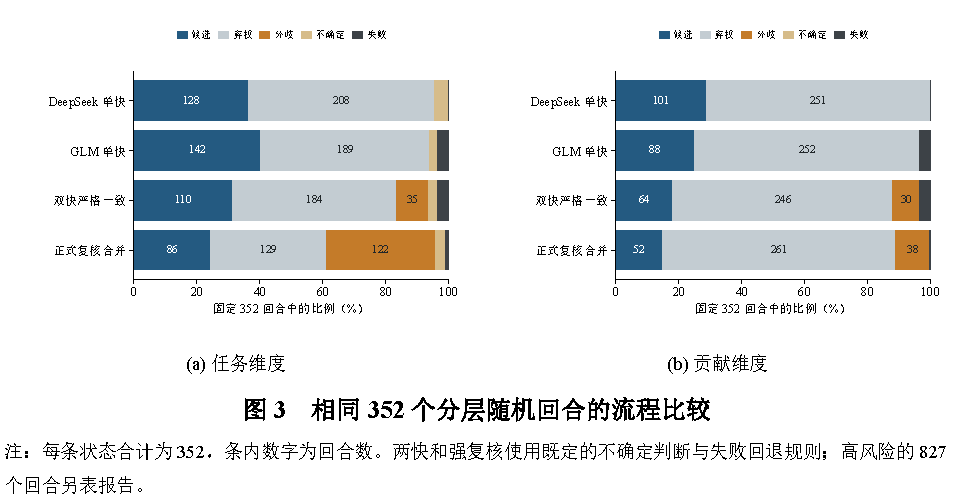
\includegraphics[width=\linewidth,height=.33\textheight,keepaspectratio]{../results/final-analysis/fig02_random_flow.pdf}
\caption{相同 352 个分层随机回合的流程比较。每条状态合计为 352；两快和强复核使用既定的不确定判断与失败回退规则。}\label{fig:flow}
\end{figure}
\begin{table}[htbp]\centering\small
\caption{共同随机集的状态计数；单模型候选不要求另一模型一致}\label{tab:flow}
\begin{tabular}{@{}llrrrrr@{}}\toprule
维度 & 流程 & 候选 & 弃权 & 分歧 & 不确定 & 失败\\\midrule
任务 & DeepSeek 单快 & 128 & 208 & 0 & 16 & 0\\
任务 & GLM 单快 & 142 & 189 & 0 & 9 & 12\\
任务 & 双快严格一致 & 110 & 184 & 35 & 11 & 12\\
任务 & 强复核合并 & 86 & 129 & 122 & 12 & 3\\
贡献 & DeepSeek 单快 & 101 & 251 & 0 & 0 & 0\\
贡献 & GLM 单快 & 88 & 252 & 0 & 0 & 12\\
贡献 & 双快严格一致 & 64 & 246 & 30 & 0 & 12\\
贡献 & 强复核合并 & 52 & 261 & 38 & 0 & 1\\
\bottomrule\end{tabular}
\end{table}
任务候选覆盖由单快的 36.36\%／40.34\%，变为双快严格一致的 31.25\% 和复核合并的 24.43\%。相对双快，复核获得 7 条新候选、撤回 31 条候选；双方都保留候选的 79 条中有 4 条改标。任务分歧由 35 增至 122，表明新增判断使部分原来的一致不再成立。贡献候选由 64 变为 52，获得 13、撤回 25；共同候选 39 条中有 5 条改标。流程选择同时改变覆盖与候选组成，无法用单一候选率评定其准确性。

与随机层相对，827 个风险回合的任务候选由双快的 39 增至复核后的 98，获得 76、撤回 17。风险层包含更集中的初始分歧与失败，复核在这里主要增加可判定结果；随机层则主要减少候选。两种方向共同说明，复核的收益依赖路由所选问题。正文后续指标使用合并后的最终候选，风险层不与随机层合并估计总体误差率。
}

\newcommand{\FinalDistributionResults}{%
\begin{figure}[htbp]\centering
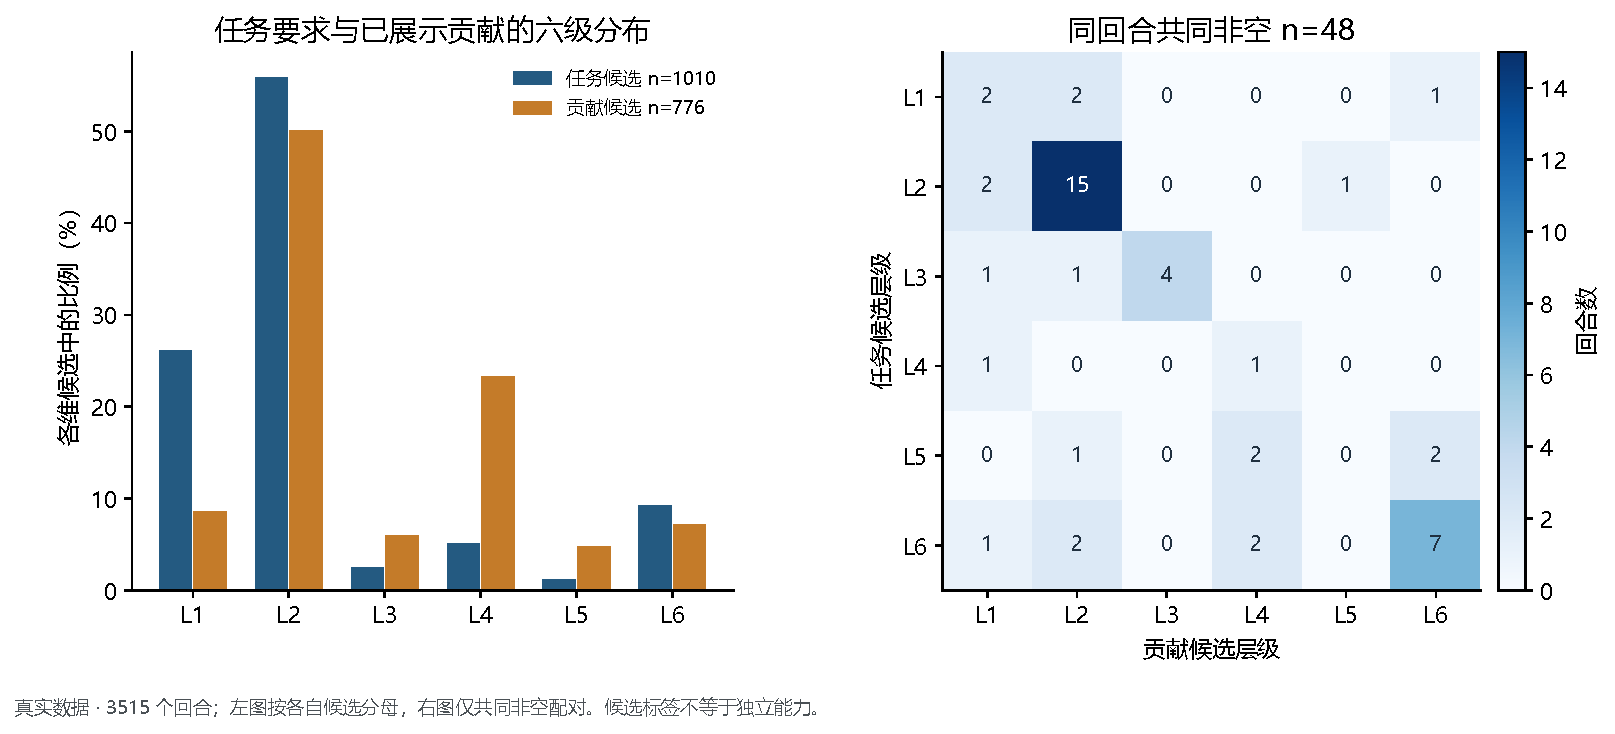
\includegraphics[width=\linewidth,height=.33\textheight,keepaspectratio]{../results/final-analysis/fig01_dimensions.pdf}
\caption{双维边际层级分布与同回合共同非空配对。左图各维按自己的候选分母；右图仅 48 个配对，颜色与数字表示回合数。}\label{fig:dimensions}
\end{figure}
\begin{table}[htbp]\centering\small
\caption{学期内候选描述；学生等权只平均该维至少有一个候选的学生—学期单元}\label{tab:description}
\begin{tabular}{@{}llrrrrr@{}}\toprule
学期 & 维度 & 候选回合 & 候选单元 & 平均层级 & 回合加权 HOT & 学生等权 HOT\\\midrule
秋季 & 任务 & 661 & 257 & 2.554 & 19.52\% & 18.58\%\\
秋季 & 贡献 & 621 & 190 & 2.953 & 37.84\% & 34.29\%\\
春季 & 任务 & 349 & 99 & 1.734 & 8.02\% & 5.56\%\\
春季 & 贡献 & 155 & 54 & 2.542 & 25.16\% & 22.57\%\\
\bottomrule\end{tabular}
\end{table}
任务候选的 L2 占主导；贡献候选则有较多 L4。边际 HOT 分别为 15.54\% 与 35.31\%，但 1010 个任务候选与 776 个贡献候选并非同一组回合，不能据两均值之差推断认知提升。在 48 个同回合共同非空配对中，任务高于贡献 13 个、相同 29 个、低于贡献 6 个，任务减贡献的平均层级差为 0.375；仅 5 个配对满足“任务为 HOT、贡献非 HOT”。共同配对只占全部回合的 1.37\%，支持的是局部双维对应关系。

表\ref{tab:description}同时改变加权单位：秋季任务 HOT 由回合加权 19.52\% 变为学生等权 18.58\%，春季由 8.02\% 变为 5.56\%。方向保持相同，但幅度变化表明较多候选回合的单元对回合加权结果贡献更大。贡献维度也有这种差异。群体报告因此同时呈现候选覆盖、回合统计和学生等权统计，并将“有候选”条件保留到结论中。
}

\newcommand{\FinalHumanResults}{%
\begin{figure}[htbp]\centering
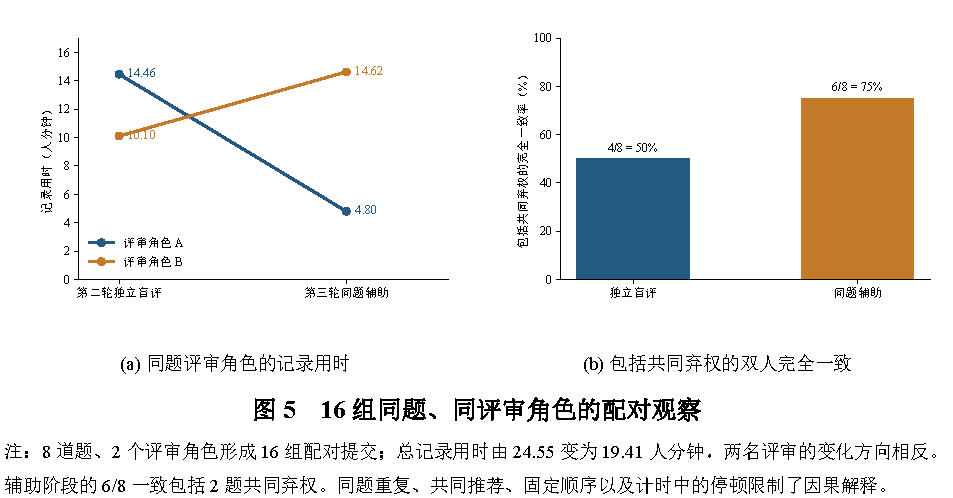
\includegraphics[width=\linewidth,height=.33\textheight,keepaspectratio]{../results/final-analysis/fig04_human_pairs.pdf}
\caption{16 组同题、同评审配对提交。两名评审的记录用时变化方向相反；辅助阶段的 6/8 一致包括 2 题共同弃权。}\label{fig:human}
\end{figure}
评审 A 的记录用时由 14.46 降至 4.80 人分钟，评审 B 由 10.10 升至 14.62 人分钟。合计减少 5.14 人分钟掩盖了个体方向差异；计时还包含停顿，因此保留逐角色数值比只报告一个效率比例更有信息。辅助后的 6 题一致中，4 题给出相同层级、2 题共同弃权，显示校准部分来自对证据不足边界的共同认识。
}

\newcommand{\FinalAssociationResults}{%
资格检查使用 3515 个真实回合，其中 1010 个任务候选；可用逐回合时间戳为 0，严格前瞻关联的合格记录为 0、学生簇为 0。CSV 创建时间虽存在，其语义不支持回合发生顺序；因此本次没有估计回归系数，设计矩阵检查止于样本资格门槛。独立学习结局、无 AI 可比对照和处理前基础也未出现在所分析资料中。
}

\newcommand{\FinalAvailabilityResults}{%
实际学生—学期共 401 个单元，其中 356 个至少有一个任务候选，45 个没有任务候选。候选支持 ABL/HOT/DHI；257 个单元满足 MAB 的字段条件，其余 99 个候选单元位于工具身份缺失的春季。有效会话边尚未核验，CTQ 可计算数为 0，完整 AIV 可计算单元数为 0，点分保持缺失。可计算子指标及缺失原因共同保留。
}

\newcommand{\FinalSensitivityResults}{%
本次求解使用联合可行集的保守外包：将 ABL/HOT/DHI 的单项改标界分别截断至 $[0,1]$，缺失指标取 $[0,1]$，再枚举权重乘子的 32 个顶点。外包保留所有满足改标预算的真实组合，同时可能包含不能共同出现的组合，故其宽度与无法区分比例具有保守性。结果仅针对 356 个有任务候选的学生—学期单元，不外推到 45 个无候选单元。
\begin{figure}[htbp]\centering
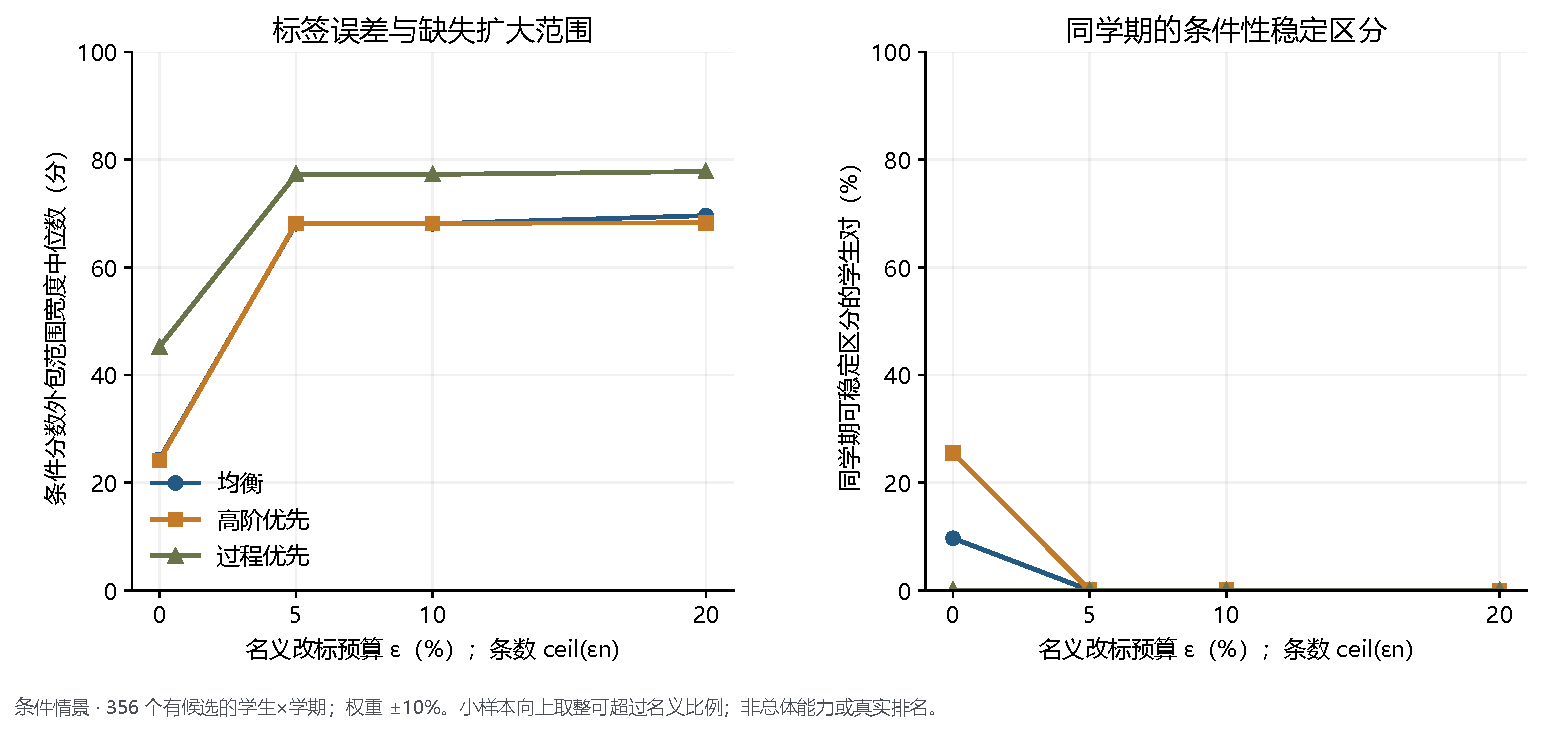
\includegraphics[width=\linewidth,height=.33\textheight,keepaspectratio]{../results/final-analysis/fig05_score_sensitivity.pdf}
\caption{真实候选单元上的条件分数外包范围。权重逐项相对扰动 $\pm10\%$；$\epsilon$ 经向上取整转为改标条数，图中稳定区分限于同学期配对。}\label{fig:sensitivity}
\end{figure}
\begin{table}[htbp]\centering\small
\caption{范围宽度和条件可区分性；356 个候选单元、37747 个同学期对}\label{tab:sensitivity}
\begin{tabular}{@{}rllrr@{}}\toprule
$\epsilon$ & 权重扰动 & 方案 & 宽度中位数（分） & 可稳定区分对数\\\midrule
0.00 & 0\% & 均衡 & 20.00 & 6228/37747\\
0.00 & 0\% & 高阶 & 20.00 & 12575/37747\\
0.00 & 0\% & 过程 & 40.00 & 0/37747\\
0.00 & 10\% & 均衡 & 24.33 & 3651/37747\\
0.00 & 10\% & 高阶 & 24.14 & 9638/37747\\
0.00 & 10\% & 过程 & 45.18 & 0/37747\\
0.05 & 10\% & 均衡 & 68.11 & 0/37747\\
0.05 & 10\% & 高阶 & 68.18 & 1/37747\\
0.05 & 10\% & 过程 & 77.27 & 0/37747\\
0.20 & 10\% & 均衡 & 69.62 & 0/37747\\
0.20 & 10\% & 高阶 & 68.29 & 0/37747\\
0.20 & 10\% & 过程 & 77.81 & 0/37747\\
\bottomrule\end{tabular}
\end{table}
不改标且固定权重时，三方案范围宽度中位数分别为 20、20、40 分；仅加入权重 $\pm10\%$ 扰动后，变为 24.33、24.14、45.18 分。可稳定区分对数分别从 6228、12575、0 降至 3651、9638、0。过程优先给缺失 CTQ 更大权重，因而真实资料不能支持该方案下的稳定区分。

名义 $\epsilon=.05$ 时，$\lceil\epsilon n_i\rceil$ 允许每单元改变 1 至 2 条标签，实际改标比例中位数为 50\%、最大为 100\%；这是候选稀疏条件下的“至少一条改标”检查。加入权重扰动后，三方案外包宽度中位数达到 68.11、68.18、77.27 分，可稳定区分对数为 0、1、0。$\epsilon=.20$ 时三方案均为 0。结果说明，低候选数、结构缺失和外包的保守性共同限制个体分数用途；它不等价于测得了相应比例的标签错误，也不证明所有学生的真实能力相同。
}

\newcommand{\FinalAttackResults}{%
\begin{table}[htbp]\centering\small
\caption{指标攻击与条件反例；均为确定性合成构造}\label{tab:attacks}
\begin{tabularx}{\textwidth}{@{}p{.15\textwidth}p{.30\textwidth}p{.21\textwidth}X@{}}\toprule
对象 & 控制条件与干预 & 数值结果 & 反馈位置\\\midrule
HOT & 标签 $[2,3,4,5]$ 复制一条 L5，保留同一认知内容 & $2/4\to3/5$，增加 0.10 & 依据来源去重，并保留真实重复练习事件\\
MAB & 同一标签，工具数由 1 增至 4 & 均衡分增加 11.39 & C：工具机会与评分权重\\
MAB 对照 & 对上述工具堆叠设 MAB 零权重 & 该攻击增分为 0 & E：同时说明广度激励的取舍\\
DHI & 按预设 $q$ 构造标签分布 & 对称／非对称均为 1 & 依据课程信息设定 $q$，解释限于分布贴合\\\bottomrule
\end{tabularx}
\end{table}
}


\title{\texorpdfstring{面向 AI 辅助学习的增量价值评价：\\认知证据、误差传播与稳健决策}{面向 AI 辅助学习的增量价值评价：认知证据、误差传播与稳健决策}}
\author{南行\\缪雨轩\quad 郭雨辰\quad 徐问天\quad 张梓涵}
\date{中国第一届数学建模黑客松｜2026 年 9 月}
\AtBeginDocument{\hypersetup{pdftitle={面向 AI 辅助学习的增量价值评价：认知证据、误差传播与稳健决策},pdfauthor={南行},pdfsubject={Math Hackathon 2026 赛道一研究论文}}}

\begin{document}
\maketitle
\begin{center}\small 南行\quad 缪雨轩\quad 郭雨辰\quad 徐问天\quad 张梓涵\\
中国第一届数学建模黑客松\quad 2026 年 9 月\end{center}
\begin{abstract}
AI 辅助学习的过程评价需要区分任务提出的认知要求、学生实际展示的认知操作，以及撤去工具后的独立学习增益。本文以两学期平台日志为对象，建立“资料—认知测量—比较资格—指标合成—反例反馈—教学行动”的统一模型。将每条学生提问编码为任务要求和已展示贡献两个维度，以弃权保留证据不足；在固定随机子集上比较单快模型、双快模型和强模型复核流程，并用同题人工独立判断与 AI 推荐辅助复评考察判定边界。随后定义五项有界指标，以三套评价权重及标签、缺失和权重扰动计算条件范围，用主动攻击检查指标与教学目标的偏离。

\FinalAbstractResults{}

在 8 道诊断题的 16 组同题、同评审角色配对提交中，AI 推荐辅助复评的双人一致由 4/8 变为 6/8，后者含 2 题共同弃权；记录用时由 24.55 变为 19.41 人分钟，两名评审的变化方向不同，结果反映同题辅助条件下的观察差异。固定标签的合成反例中，工具堆叠使均衡分数增加 11.39 分，说明工具广度的评分作用需要机会条件和反例检验。现有日志支持过程诊断与条件范围；独立学习结局及有效回合时间的缺失，分别限制因果估计和滞后关联。评价链据此把结果转为可追溯的教学建议与数据补采要求。
\keywords{AI 辅助学习；认知测量；选择性标注；复合指标；敏感性分析；教学决策}
\end{abstract}

\section{问题与研究思路}
学生向 AI 请求“比较两个方案”，与学生自己完成比较，属于不同的认知证据。工具使用频次、生成答案的质量和学生离开工具后的学习表现，也处在不同的测量层面。认知投入框架强调可观察活动的差异，认知卸载与 AI 素养研究则提示工具使用需要结合人的判断过程解释\cite{chi2014_icap,risko2016_offloading,long2020_literacy}。因此，本文围绕一个问题展开：\textbf{怎样把可核对的过程证据转成能够说明适用条件、经得起反例检验的学习诊断？}

赛题的五个模块对应一条相互约束的研究链。A 从原文形成认知候选及其不确定性；B 确定候选能够支持的比较；C 将可用测量转成指标和条件分数；D 检验标签、权重及行为操纵能否改变结论；E 将稳定结论和不确定来源映射为教学行动。设原始记录和来源坐标为 $(R,P)$，两维标签为 $(L^T,L^C)$，可比较集合为 $\mathcal P$，指标为 $x$，分数为 $S$，则
\begin{equation}\label{eq:chain}
(R,P)\longrightarrow(L^T,L^C,U_L)\longrightarrow\mathcal P
\longrightarrow(x,U_x)\longrightarrow(S,U_S)\longrightarrow a.
\end{equation}
$U_L,U_x,U_S$ 分别保存标签、指标和分数的不确定性。D 的检验沿相反方向反馈：证据匹配问题修订 A 的标注条件，时间或样本选择问题缩小 B 的比较范围，刷分与权重敏感性修订 C 的解释及 E 的行动强度。

\begin{figure}[htbp]
\centering
\begin{tikzpicture}[node distance=0.36cm,>=Stealth,
box/.style={draw,rounded corners=2pt,align=center,font=\small,text width=2.25cm,minimum height=1.13cm},
flow/.style={->,thick}]
\node[box] (a) {A 认知测量\\任务／贡献／弃权};
\node[box,right=of a] (b) {B 比较资格\\选择／时间／结局};
\node[box,right=of b] (c) {C 指标合成\\定义域／条件范围};
\node[box,right=of c] (d) {D 反例检验\\扰动／攻击／回验};
\node[box,right=of d] (e) {E 教学行动\\建议／补采条件};
\draw[flow] (a)--(b);\draw[flow] (b)--(c);\draw[flow] (c)--(d);\draw[flow] (d)--(e);
\draw[flow] (d.south)--++(0,-.7)-|node[pos=.50,below,font=\small]{检验结果反馈到测量、可比性与指标定义}(a.south);
\draw[flow] (d.south)++(0,-.7)-|(b.south);
\draw[flow] (d.south)++(0,-.7)-|(c.south);
\end{tikzpicture}
\caption{证据进入评价链，反例沿链反馈；每一环节向下游传递结果及适用条件。}\label{fig:chain}
\end{figure}

本文的方法选择服务于上述接口。LLM 评审研究表明，提示设计、重复运行与文本攻击会改变判断\cite{gu2026_judge_survey,haldar2025_inconsistency,yamauchi2025_design,zhao2025_onetoken}；本文据此同时保留弃权、有效分母和复核来源。预测辅助推断可用概率抽取的参考标签校正群体均值，但收益依赖残差和抽样条件\cite{angelopoulos2023_ppi,angelopoulos2024_ppiplus,mani2025_nofreelunch}；本文将其作为校验资源配置的设计依据。教育效果研究将工具辅助表现与独立学习结局分开\cite{bastani2025_guardrails,he2024_metaanalysis}；本文相应把过程描述与因果目标分开建模。复合指标中的缺失、权重和排序不确定性按统一的可行范围处理\cite{oecd2008_composite}。

\section{资料、研究单位与选择机制}
\subsection{研究总体与来源连接}
资料包含 2025 年秋季与 2026 年春季平台问答表，以及秋季智能体使用表。两学期问答表共 2770 行；按学期窗口、春季参与名册和文本可用性筛选后纳入 1225 行，其中秋季 824 行、春季 401 行。排除条件存在重叠，筛选后的数量以实际交集计数。在这些行内按 Q/A 结构恢复 3522 个学生提问回合，其中 3515 个满足送评结构条件，构成本文的真实分析总体；另外 12 条合成控制仅用于流程检查。

回合、原始 CSV 行、会话和学生—学期是不同单位。每个回合保留源文件哈希、行号、字段内字符区间和片段标识。回合顺序由文本结构恢复，CSV 创建时间表示原始行的记录时间；二者均不直接给出逐回合发生时间或已经核验的会话相邻边。跨学期学生标识按学生—学期单元处理，未经身份连接验证的标识不作为纵向同一人。公开图表采用聚合结果，逐条文本与来源保存在授权私有资料中。

\begin{table}[htbp]\centering\small
\caption{真实总体与两维最终候选的分母}\label{tab:population}
\begin{tabular}{@{}lrrrr@{}}\toprule
学期 & 入选原始行 & 合格学生回合 & 任务候选 & 任务候选覆盖\\\midrule
2025 秋 & 824 & 2509 & 661 & 26.35\%\\
2026 春 & 401 & 1006 & 349 & 34.69\%\\
合计 & 1225 & 3515 & 1010 & 28.73\%\\\bottomrule
\end{tabular}
\end{table}

\subsection{可判定性是分析结果的一部分}
记 $O_i^T,O_i^C$ 为任务和贡献维度存在最终候选的指示，$O_i^E,O_i^M$ 为会话边与工具字段满足定义要求的指示。任务候选仅占总体的 28.73\%，因此候选中的层级均值回答的是“可判定文本表现出什么特征”。对有界目标量 $Z$，有
\begin{equation}\label{eq:selection}
\E[Z\mid O=1]-\E[Z]=\frac{\Cov(Z,O)}{P(O=1)}.
\end{equation}
当文本长度、表达方式或任务复杂度同时影响 $Z$ 与可判定性时，候选分布便具有选择性。两学期候选覆盖相差 8.34 个百分点，比较均值前必须先检查两者究竟筛选了什么。弃权是证据不足的判断，分歧是有效判断未形成一致，技术失败是请求或输出不可用；三者对后续补采和人工处理的意义不同。

\FinalSelectionResults{}

\section{A：认知测量与 AI 辅助校验}
\subsection{两维标签、决策规则与共同样本比较}
L1 至 L6 依次表示记忆、理解、应用、分析、评价、创造。任务标签 $L^T$ 编码学生原文要求执行的操作；贡献标签 $L^C$ 编码学生本人已经展示的操作。只提出一个分析问题可以提供任务维度证据，而贡献维度需要可见的分析内容。证据不足时输出 $\bot$，与 L1 分开记录。模型同时返回连续原文、判断理由和状态；逐字符引文匹配核验的是来源位置，语义层级由模型与人工分别判断。

两快模型独立处理全部 3515 回合。按学期、种子 26 预选 352 回合（秋季 251、春季 101）接受两强模型独立复核；另有 827 回合由分歧、失败或解析风险等条件进入风险复核。首次复核不提供快模型答案。比较流程时固定在相同 352 个随机回合上：单快流程接受单模型有效判断；双快流程按两模型规则形成候选；强复核流程按已执行的复核规则再形成结果。这样得到的是同一输入集合上覆盖、弃权与分歧的代价，而非把风险子集和全量简单比较。

设模型接受指示为 $A_{im}$，覆盖为 $c_m=N^{-1}\sum_iA_{im}$。独立参考标签 $Y_i$ 存在时，条件错误风险定义为
\begin{equation}\label{eq:risk}
R_m=\frac{\sum_i A_{im}\ind(\widehat L_{im}\ne Y_i)}{\sum_i A_{im}}.
\end{equation}
本次共同随机集保留模型之间的一致性与状态比较；没有以模型多数票构造式\eqref{eq:risk}中的独立参考。Cohen $\kappa=(p_o-p_e)/(1-p_e)$ 使用共同非空配对，区间按学生整簇重抽样。共同弃权另列，避免以大量共同未知掩盖可判定部分的差异。

\FinalWorkflowResults{}

\subsection{真实双维分布与层级解释}
在完整的 3515 回合中，任务维度有 1010 个最终候选、1812 个一致弃权、604 个分歧、76 个不确定和 13 个技术失败；贡献维度分别为 776、2457、268、0 和 14。任务与贡献的覆盖分别为 28.73\% 和 22.08\%，贡献维度的一致弃权达到 69.90\%。因此，平台保留的学生文本对“提出了什么要求”的证据多于“实际完成了什么操作”的证据。两维候选必须分别描述；其覆盖差不能直接解释为学生认知水平的差距。

\FinalDistributionResults{}

两快模型任务维度共同非空 1248 对，六级 $\kappa=0.795$，学生整簇重采样 95\% 区间为 $[0.764,0.826]$；贡献维度共同非空 955 对，$\kappa=0.644$，区间 $[0.602,0.682]$。学生簇重抽样保留同一学生内部依赖；跨学生共享缓存仍产生簇间依赖，这部分未在区间中额外校正。贡献判断的分歧更大，与其需要额外识别“学生是否实际展示操作”的要求相符。该解释是一种与测量定义一致的观察，并未将两维差异分解为模型能力或任务难度的因果作用。固定 40 回合的重复检查中，两快模型各有 39 个双有效配对，任务重复相同分别为 36/39、35/39，贡献均为 35/39；重复性为下游标签扰动提供了必要性依据。

\subsection{独立判断到 AI 推荐辅助复评}
人工小样本以判定边界诊断为目标。首轮收集 12 份独立提交；随后两名评审对固定的 8 道诊断题各独立提交一次，共 16 份。AI 将判断说明组织为“主要操作—对象或条件—证据—边界”四个部分；在同一 8 题上显示共同推荐后，两名评审再各提交 8 份。两阶段按评审和题目连接，形成 16 组提交配对。原始独立判断、推荐快照、辅助修改和记录用时分别保存；最终 4 份定点人工核验另行封存。

\begin{table}[htbp]\centering\small
\caption{同题独立判断与 AI 推荐辅助复评；8 题、2 名评审}\label{tab:human}
\begin{tabular}{@{}lcc@{}}\toprule
观察量 & 独立阶段 & 推荐辅助阶段\\\midrule
提交数 & 16 & 16\\
双人完全一致（含共同弃权） & 4/8 & 6/8\\
双方均给出层级 & 7/8 & 6/8\\
双方共同弃权 & 0/8 & 2/8\\
HOT 一致（双方给层级） & 4/7 & 5/6\\
六级 $\kappa$（双方给层级） & 0.344 & 0.556\\
连续原文证据匹配 & 16/16 & 16/16\\
记录用时合计（人分钟） & 24.55 & 19.41\\\bottomrule
\end{tabular}
\end{table}

\FinalHumanResults{}

原独立阶段的 4 道分歧题在辅助阶段形成一致，但有 2 道原先一致的题转为分歧，其中一题跨越 L3/L4 的 HOT 边界。13/16 份辅助标签与推荐相同，9/16 份的标签、证据和理由逐字相同；这说明推荐实际进入了判定过程，也说明共同推荐会改变评审间依赖关系。人工先判断后再看建议仍可能受锚定影响\cite{bucinca2021_forcing,ashktorab2024_reliance}。故表\ref{tab:human}描述的是小样本同题辅助复评：题目熟悉、填写减少和推荐锚定均可能参与观察差异。末轮 4 份核验保留其辅助裁定身份，未回写两阶段的一致性分母。

这项探索对 A 与 C 的直接反馈是：判断协议必须同时呈现层级依据和不可判定边界；三阶分组 L1--2、L3--4、L5--6 的一致仍可能掩盖 HOT 所使用的 L3/L4 分界。因此，群体报告保留六级分布、HOT 与共同弃权，个体建议优先回查能改变行动的边界分歧。

\section{B：可比性、过程关联与增量目标}
\subsection{从已观测对象定义估计目标}
模块 A 输出的是筛选后的认知候选。B 首先检查学期、课程、工具机会、学生组成与时间信息，确定这些候选支持何种比较。秋季与春季的任务候选覆盖分别为 26.35\% 和 34.69\%；春季工具身份字段不可直接核实。由此，两学期的原始分布差同时混合了任务内容、可判定性与观测机会差异。本文保留学期内描述以及共同定义下的分布比较，将其解释为日志的过程特征。

若研究 AI 对独立学习的增量，设事前定义的干预为 $T_i\in\{0,1\}$，共同量尺、撤去工具后的潜在结果为 $Y_i(t)$，目标量为
\begin{equation}\label{eq:ate}
\tau_{\mathcal P}=\E[Y_i(1)-Y_i(0)\mid i\in\mathcal P].
\end{equation}
识别需明确干预版本、时间零点、前测基础 $X$、课程条件 $C$ 和工具机会 $A$，并满足一致性、条件交换性 $(Y(1),Y(0))\perp T\mid X,C,A$ 与共同支持等条件\cite{hernan2020_whatif}。对照、失访和支持集可作资料诊断；未测混杂的影响仍需敏感性分析\cite{lu2023_sensitivity}。

\subsection{实际资格检查与未识别来源}
\FinalAssociationResults{}

可执行的过程关联以更早的候选历史预测更晚的任务或贡献候选。对回合 $t$，令 $n_{i,<t}$ 为严格较早且可判定的回合数，$H_{i,<t}$ 为其中 HOT 比例，可考虑
\begin{equation}\label{eq:association}
Z_{it}=\beta_0+\beta_1\log(1+n_{i,<t})+\beta_2H_{i,<t}
+\gamma_{\mathrm{term}}+\eta\,\mathrm{time}_{it}+u_{it},
\end{equation}
并按学生—学期单元聚类。$n_{i,<t}$ 只计入可判定历史，解释为标签可见的过程累积；它不等于全部 AI 使用量。设计门槛为至少 100 条具有前序历史的记录、30 个学生簇及满秩设计矩阵。门槛用于阻止结构上无法估计的拟合，不构成统计功效保证。由于本次逐回合时间不可用，式\eqref{eq:association}停留在已定义而未获得合格样本的过程模型。

对独立学习增量，结局缺失具有更强的限制。
\begin{proposition}[独立结局缺失下的不可识别性]\label{prop:noid}
若资料只含使用记录 $T$、问答日志 $R$ 与课程/学期信息 $C$，且没有经验证的 $R\mapsto Y$ 测量关系，则 $\tau_{\mathcal P}$ 不能由这些观测变量点识别。
\end{proposition}
\begin{proof}
固定任意观测分布 $P(T,R,C)$。第一种机制令 $Y(0)=Y(1)=0$；第二种机制令 $Y(0)=0,Y(1)=1$。两者对观测资料给出完全相同的分布，目标效应却分别为 0 与 1。因此观测资料不能唯一确定该效应。其他有界结果尺度可取两个不同常数作同样构造。
\end{proof}

该结论给出后续采集的优先顺序：独立前后测及共同锚定任务用于确定结果尺度，处理前基础和工具机会用于建立比较人群，逐回合时间和核验会话边用于过程动态分析。人工标签复评衡量的是标注过程，不是学生学习前后测。B 将这些资格检查传给 C，使过程指标与学习效应保持不同的解释对象。

\section{C：有界指标与真实条件范围}
\subsection{五项指标的定义与性质}
对学生 $i$ 在固定学期窗内的 $n_i>0$ 个任务候选，记层级为 $L_{ij}\in\{1,\ldots,6\}$，六级经验分布为 $p_i$。平均层级与高阶占比定义为
\begin{equation}\label{eq:ablhot}
x_i^{\ABL}=\frac{n_i^{-1}\sum_jL_{ij}-1}{5},\qquad
x_i^{\HOT}=n_i^{-1}\sum_j\ind(L_{ij}\ge4).
\end{equation}
ABL 反映整体层级，HOT 关注分析及以上的份额；二者来自同一标签，相关性在合成中保留。

令 $E_i$ 为经核验的同一会话内相邻学生回合边，边端点为 $e^-,e^+$。当 $|E_i|>0$ 时，认知跃迁指标为
\begin{equation}\label{eq:ctq}
x_i^{\CTQ}=\frac12+\frac{\sum_{e\in E_i}(L_{e^+}-L_{e^-})}{10|E_i|}.
\end{equation}
该值衡量净方向，升降相抵会隐藏探索路径，故具备边资料时还需报告上升、下降和持平边。无有效边时 CTQ 未定义。

预设教学目标分布 $q=(.10,.15,.20,.25,.20,.10)$，以总变差定义分布贴合度：
\begin{equation}\label{eq:dhi}
x_i^{\DHI}=1-\frac12\sum_{k=1}^6|p_{ik}-q_k|.
\end{equation}
$q$ 代表课程设计偏好。提高某一个层级未必增加贴合度，过量集中于任一级都可能远离目标。针对低层过量的非对称敏感性方案为
\begin{equation}\label{eq:dhia}
\begin{split}
d_a(p,q)&=\sum_{k=1}^5\left[2\{F_p(k)-F_q(k)\}_++\{F_q(k)-F_p(k)\}_+\right],\\
x_i^{\DHI_a}&=1-d_a(p_i,q)/M(q),\qquad M(q)=\max_{j=1,\ldots,6}d_a(e_j,q).
\end{split}
\end{equation}
$F$ 为累计分布，$2{:}1$ 惩罚比作为明示偏好参与扰动。若工具身份完整，$m_i$ 为实际不同工具数，工具广度为
\begin{equation}\label{eq:mab}
x_i^{\MAB}=\min\{1,\log(1+m_i)/\log5\}.
\end{equation}
工具身份缺失对应未知，原始 $m_i$ 与课程可用工具数同时进入解释。

\begin{proposition}[有界性与边集合稳定性]\label{prop:bounds}
五项归一指标在各自定义域内属于 $[0,1]$。CTQ 在有效边集合固定时按边数加权分块保持不变；删除原边的比例为 $r<1$ 且保留非空边集时，新旧 CTQ 的差至多为 $r$。非对称 DHI 当且仅当 $p=q$ 时取 1。
\end{proposition}
\begin{proof}
ABL 由 $[1,6]$ 线性映射，HOT 是比例。CTQ 为每条边分数 $1/2+(L_{e^+}-L_{e^-})/10\in[0,1]$ 的平均，故分块加权不变；删除边后原均值为 $(1-r)\mu_{\rm keep}+r\mu_{\rm drop}$，差不超过 $r$。总变差不超过 1。$d_a(\cdot,q)$ 为凸函数，由 $p=\sum_jp_je_j$ 得 $d_a(p,q)\le\sum_jp_jd_a(e_j,q)\le M(q)$；各累计差为零等价于 $p=q$。MAB 经截断位于 $[0,1]$。
\end{proof}

\subsection{合成偏好与部分观测}
给定五维完整向量 $x_i$，定义
\begin{equation}\label{eq:aiv}
S_i(w)=100w^\mathsf Tx_i,\qquad w_k\ge0,\quad\sum_kw_k=1.
\end{equation}
使用表\ref{tab:weights}的三套预设偏好。它们分别强调均衡、高阶占比和过程跃迁；在没有独立学习结局时，权重表达评价取向。
\begin{table}[htbp]\centering\small
\caption{三套合成权重}\label{tab:weights}
\begin{tabular}{@{}lccccc@{}}\toprule
方案 & ABL & HOT & CTQ & DHI & MAB\\\midrule
均衡 & .20 & .20 & .20 & .20 & .20\\
高阶优先 & .10 & .50 & .20 & .15 & .05\\
过程优先 & .10 & .20 & .40 & .25 & .05\\\bottomrule
\end{tabular}
\end{table}

\FinalAvailabilityResults{}

缺失正权重指标时点分保持空值。对情景范围，则允许未观测但有界的指标在 $[0,1]$ 内变化。以已知 ABL/HOT/DHI、CTQ 缺失而 MAB 已知的单元为例，仅 CTQ 未知就使均衡、高阶、过程优先分数分别具有至少 20、20、40 分的可行宽度；MAB 同样未知时，下限宽度变为 40、25、45 分。它们由权重与定义域直接给出，提示会话边资料对“过程优先”的信息价值尤为明显。区间仍需联合考虑 ABL/HOT/DHI 的同源标签约束。

\subsection{标签与权重扰动的求解及结果}
设候选标签向量为 $\ell_i$，允许至多 $b_i=\lceil\epsilon n_i\rceil$ 个候选改标。由同一改标向量同时重算 ABL/HOT/DHI，定义
\begin{equation}\label{eq:jointset}
\mathcal U_i(\epsilon)=\left\{g(\ell_i',E_i,m_i):\sum_r\ind(\ell'_{ir}\ne\ell_{ir})\le b_i,
\ \ell'_{ir}\in\{1,\ldots,6\}\right\}.
\end{equation}
缺字段指标按明示边界扩展该集合。$\epsilon$ 表示敏感性情景，不由模型自报概率替代真实错标率。以第 $j$ 套权重为中心，逐项相对扰动后重新归一得到 $\mathcal W_j$，条件范围为
\begin{equation}\label{eq:interval}
[L_{ij},U_{ij}]=\left[\inf_{x\in\mathcal U_i,w\in\mathcal W_j}100w^\mathsf Tx,
\sup_{x\in\mathcal U_i,w\in\mathcal W_j}100w^\mathsf Tx\right].
\end{equation}
它表示指定标签、缺失及权重情景下的可行分数，不是抽样置信区间。只有两对象在同一比较条件下满足 $L_{ij}>U_{kj}$，才可判为稳定高于；重叠时保留无法稳健区分的状态。

\FinalSensitivityResults{}

固定 $n$ 条中改变 $s$ 条标签时，ABL、HOT、对称 DHI 的绝对变化均不超过 $s/n$；固定 $x\in[0,1]^5$ 且两权重和均为 1，有更紧的权重界
\begin{equation}\label{eq:bound}
|S(w,x)-S(w',x')|\le100\sum_kw_k|x_k-x'_k|+50\|w-w'\|_1.
\end{equation}
第二项利用权重差总和为零：正差与负差各占其 $L_1$ 范数的一半。该外界便于检查数值求解，但联合可行集保留指标由同一标签生成的依赖；本次报告的外包范围放松该依赖，其保守性随结果一并解释。在这些条件情景下计算的宽度及重叠情况决定 E 采用具体反馈、敏感提示还是补采行动。

\section{D：主动检验与上游反馈}
\subsection{认知目标与可操纵分数的分离}
攻击实验保持已知条件，单独改变一种输入，以定位失效机制。HOT 检验重复高阶记录对占比的影响，MAB 检验没有新增认知证据的工具堆叠，DHI 检验朝固定目标分布填充标签能否提高贴合分。攻击输入是合成计算性反例，其作用是检验指标性质。

\FinalAttackResults{}

对固定标签 $[2,3,4,5]$，仅将工具数从 1 堆到 4，均衡分数增加
\begin{equation}\label{eq:attack}
100\times0.20\left(1-\frac{\log2}{\log5}\right)=11.39\text{ 分（约）}.
\end{equation}
工具饱和映射降低了进一步增加工具的边际收益，却仍奖励从 1 到 4 的堆叠。MAB 零评分权重的对照使此攻击增分为零，同时放弃对真实有益工具广度的奖励。据此，将 MAB 作为诊断信息，并结合可用工具机会解释其评分作用。

HOT 的问题回到 A 的研究单位与 C 的分母：相同学习事件重复导出应按来源去重，真实反复练习则保留事件身份；仅凭文本相同不足以区分两者。DHI 的问题回到教学设计：$q$ 应由课程任务结构确定，达到 $q$ 只表示分布贴合。CTQ 的问题回到 B 的会话资格：切分或复制改变边集时，固定边集的不变性命题不再适用。这样，每项失败都有明确的测量或定义修订位置。

既有文本检验使用 Claude Sonnet 5、Gemini 2.5 Pro 和 DeepSeek V4.1 Flash，在 7 个合成条件下每模型各调用一次，共 21 个输出。基线和认知动词注入条件均被三个模型标为 L2；文本重复条件依次为 L1、L2、L2，HOT 均未升高。加入实质分析内容的对照则均为 L4。该小规模观察说明，在所测试文本中，仅增加动词或重复没有产生高阶标签；它与表\ref{tab:attacks}中“直接重复已有高阶标签会提高 HOT”的计算结果对应不同环节：前者检验 A 的文本编码，后者检验 C 的聚合分母。原提示、模型组合和输入规模单列保存，其结果不并入 t3 的流程比较。

\subsection{校验预算与真实证据的后续连接}
群体均值校正需与抽样设计相容。若全体具有固定预测 $f_i$，在互斥层 $h$ 内以已知概率抽得参考值 $y_i$，残差校正为
\begin{equation}\label{eq:ppi}
\widehat\mu=\frac1N\sum_if_i+\sum_hW_h\overline{(y-f)}_h,\qquad
\widehat V\approx\sum_hW_h^2\left(1-\frac{n_h}{N_h}\right)\frac{s_{r,h}^2}{n_h}.
\end{equation}
预算 $B$、单次成本 $c_h$ 下，整数分配最小化该方差并满足 $\sum_hc_hn_h\le B$，连续近似为 $n_h\propto W_h\sigma_{r,h}/\sqrt{c_h}$。合成有限总体对照验证了该配置程序，数值与条件列于附录\ref{app:simulation}。当前 352 个随机复核的参考仍为模型，定向人工题又用于边界诊断，因此式\eqref{eq:ppi}尚未产生真实总体的人工校正均值。此区分把已完成的流程比较与将来独立参考资源的配置连接起来。

\section{E：真实诊断与教学行动}
模块 E 以 A 的可见证据、B 的比较资格及 C/D 的敏感性作为输入。已上线工作台（\url{https://math.hnnu.team/}）完成资料导入、来源定位、状态检查和确定性指标计算；报告将候选来源、覆盖与缺失一并呈现。既有模型候选注明批次来源，演示输入的指标计算与解释使用明确的可用字段。教师从群体分布定位任务设计和证据采集的不足，学生获得对应原文的一项可执行反馈，运营人员负责补足导致结果不可判断的字段。

\begin{table}[htbp]\centering\small
\caption{真实结果、教学行动及适用条件}\label{tab:decision}
\begin{tabularx}{\textwidth}{@{}p{.29\textwidth}XX@{}}\toprule
本研究的观察 & 对应教学行动 & 行动的适用条件\\\midrule
贡献候选 776/3515，贡献一致弃权 2457/3515 & 在请求答案后增加学生独立解释、比较依据或修订理由的留痕环节 & 将未展示视为证据缺口；新内容由学生实际完成\\
学期任务候选覆盖 26.35\% 与 34.69\% & 分学期显示覆盖与分布，设置共同锚定任务后再比较 & 同任务、同机会、同标注口径，并检查选择性缺失\\
同题辅助复评一致 4/8 变为 6/8，仍含 HOT 边界分歧 & 使用四段判定卡；优先核查能改变教学反馈的边界题 & 保留独立与推荐辅助阶段身份，复核原文依据\\
真实 CTQ 缺失，完整 AIV 无点值 & 优先补充核验会话边；显示子指标与条件范围 & 新字段具备来源和时间语义，范围在同一情景下比较\\
工具堆叠产生 11.39 分合成增量 & 同时呈现工具机会、工具数及 MAB 的权重敏感性 & 检查广度是否对应新的认知证据与课程要求\\\bottomrule
\end{tabularx}
\end{table}

以缺少会话边的输入为例，系统可以计算候选标签的 ABL/HOT/DHI，并返回 CTQ 的缺失原因及三权重的条件范围。教师因而能够选择补充会话证据或开展共同任务，学生仍能获得针对可见文本的反馈。由此，缺失状态参与下一步行动，而不被压缩为一个难以解释的低分。可复现实现把固定输入、分析代码与聚合图表连接到同一版本，运行入口见附录\ref{app:repro/protocol}。

\section{讨论与结论}
真实资料呈现三个相互关联的结果。首先，认知需求比学生贡献更容易在提问文本中形成候选，且两者都具有明显选择性；记录学生自己的解释过程，比进一步细化一个低覆盖候选均值更能改善测量对象。其次，AI 推荐辅助复评改变了双人一致和记录用时，也产生新的边界分歧；其价值在于让判断依据可检查，作用仍依赖题目、评审和推荐条件。再次，完整 AIV 的缺失和条件范围的宽度揭示了数据瓶颈，指标攻击则揭示了目标瓶颈：更多数据与更复杂合成都需要与明确的认知目标相连。

本文形成的闭环是：双维候选连同弃权进入测量；学期选择、时间和独立结局决定比较资格；有界指标将观测与缺失转成条件范围；扰动和攻击反馈到来源单位、权重及行动规则。其数学结果包括独立结局缺失下的不可识别构造、指标有界性、CTQ 的边集稳定性和标签/权重扰动界；实证结果包括共同随机集上的流程对照、双维与学期分布、同题人工辅助观察以及真实学生—学期的可计算性和敏感性。

主要限制集中在四处：日志只覆盖筛选后文本事件，候选可判定性与研究对象相关；模型可能共享错误，小范围定向人工复评未提供总体误差率；回合时间、核验会话边和部分工具字段缺失；课程目标分布及权重具有价值选择。对应的研究升级是概率抽取的独立参考、共同锚定任务、明确的过程时间与无 AI 独立结局。现阶段的教学使用据此定位于可追溯的过程诊断、边界复核和补采决策。

\noindent\textbf{AI 使用声明。}AI 用于文献整理、代码与推导辅助、两维认知编码、推荐辅助复评及图文表达。批量测评、人工独立判断、辅助采纳和最终核验分别保存，团队负责公式、文献、结果解释与提交。工具身份、调用与采用过程详见附录\ref{app:ai}。

\begingroup
\linespread{1.15}\selectfont
\AtNextBibliography{\interlinepenalty=10000}
\printbibliography[title={参考文献}]
\endgroup
\clearpage
\appendix
\pagenumbering{arabic}
\renewcommand{\thepage}{附-\arabic{page}}
\renewcommand{\thesection}{\Alph{section}}
\renewcommand{\thesubsection}{\Alph{section}.\arabic{subsection}}
\titleformat{\section}{\centering\heiti\zihao{3}\bfseries}{附录\thesection}{0.8em}{}
\section{研究对象、计算细节与仓库复现}\label{app:repro/protocol}
\subsection{主要符号与结果入口}
\begin{longtable}{@{}p{.20\textwidth}p{.73\textwidth}@{}}
\caption{主要符号及计算对象}\\\toprule 符号 & 含义\\\midrule\endfirsthead
\toprule 符号 & 含义\\\midrule\endhead
$R,P$ & 原始资料及文件、行、片段、位置索引。\\
$L^T,L^C,\bot$ & 任务要求、已展示贡献与证据不足的弃权。\\
$O^T,O^C,O^E,O^M$ & 两维候选、核验会话边和工具字段的可用指示。\\
$Y(1),Y(0),\tau$ & 无 AI 独立测量的潜在结果与目标因果效应。\\
$p_i,q,E_i$ & 学生候选层级分布、预设课程分布和核验相邻边。\\
$x_i,w,S_i$ & 五指标、非负和为一的权重、完整条件下的点分。\\
$\epsilon,b_i,\mathcal U_i,\mathcal W_j$ & 名义改标参数、整数改标条数、联合指标及权重集合。\\
\bottomrule
\end{longtable}

主结果为逐回合批次 t3。冻结清单位于
\begin{center}\small\path{runtime/research/full-turns-v1-20260926T143225Z/t3/frozen/snapshot-manifest.json}\end{center}
其 SHA-256 为\par\noindent\small\path{7e885ceecf12a180349369ed9ddfc962ad71f1ea270f68b037a86a396430631d}\normalsize\par
聚合分析入口为 \path{results/final-analysis/summary.json}，其中保存输入哈希、分母、方法条件、分析代码哈希和图表索引。论文所用聚合段落与表格在 \path{paper/final_analysis_results.tex}；图表由实际分析结果绘制。源文件、结果与最终 PDF 的哈希由交付清单绑定，代码版本使用仓库交付说明中的固定提交。

\subsection{来源、输出状态和统计分母}
两学期 2770 条问答行经范围筛选得到 1225 行，在其中恢复 3522 个学生提问回合，合格文本回合 3515。结构异常的 7 回合保留来源，不进入模型统计。DOCX 正文、图片及转写另有来源清单，未经验证的跨文件身份与会话连接不参与本研究的统一计数。学生—学期表保留 401 个单元；只有具有任务候选的 356 个单元进入候选指标敏感性，其他 45 个单元保留无候选状态。

基础逻辑任务为 $3515\times2=7030$，有效输出 6929，失败 101；有效包括明确弃权。随机复核为 352 回合、704 个逻辑任务，其中有效 692；额外风险复核为 827 回合、1654 个逻辑任务，其中有效 1638。12 个合成控制产生 48 个有效基础/复核输出；两快模型各 40 个重复任务，共 80 个，其中有效 78。真实 API 尝试、重试、逻辑任务和真实学生样本分别计数。相同输入仅在实验、模型、阶段、提示和参数完全相同时复用校验成功的响应；重复性检查不复用首次响应。

按维度先形成双模型状态：所需输出缺失记技术失败；两标签（含空值）不同记分歧；共同空值记弃权；任务维度共同非空但任一输出标为不确定时保留不确定；其余相同非空标签形成候选。已复核回合优先采用两强模型的候选或共同弃权；只有强复核技术失败、而双快已有候选或共同弃权时，回退双快结果。强模型之间的分歧继续保留。该规则逐条与封存最终状态核对，相同随机集流程比较使用同一套规则。

两模型六级一致性只用双方非空记录，三阶将 L1--2、L3--4、L5--6 合并。学生整簇重抽样次数为 2000，保留同一学生内部依赖；跨学生共享缓存造成的簇间依赖未在这些区间中额外校正。同模型重复、共享缓存与同题辅助复评均保留记录身份和来源。随机层与风险层分别列示，风险层用于定位难例，不能按其比例推断全体错误率。

\subsection{敏感性计算的定义域}
全回合未知标签范围固定所有最终候选，把其他回合分别赋予允许的最低与最高值。若总回合为 $N$、候选数为 $n$、候选层级和为 $s$、候选高阶数为 $h$，则
\begin{equation}
\mathrm{ABL}_{\rm raw}\in\left[\frac{s+N-n}{N},\frac{s+6(N-n)}{N}\right],\qquad
\HOT\in\left[\frac hN,\frac{h+N-n}{N}\right].
\end{equation}
该构造假设未知回合具有潜在六级值，评价的是这一假设下的敏感性；它没有把弃权重新认定为已观测标签。春减秋范围采用春季下界减秋季上界及春季上界减秋季下界。

学生分数范围的对象是具有候选的学生—学期单元。允许改标条数取 $b_i=\lceil\epsilon n_i\rceil$，取 $\epsilon=0,.05,.10,.20$。实现用 ABL/HOT/DHI 各自变化不超过 $b_i/n_i$ 的区间，截断至 $[0,1]$；缺失 CTQ/MAB 取 $[0,1]$。这些边际区间的笛卡尔积是式\eqref{eq:jointset}的保守外包，允许部分不能同时出现的指标组合。权重乘子为 $1\pm .10$，枚举五项乘子的 32 个顶点后归一；对外包矩形在每个顶点求线性极值，得到外包范围。区间不重叠是稳定区分的充分条件；重叠可能来自实际不确定性，也可能来自外包的保守性。

同学期比较共 $\binom{257}{2}+\binom{99}{2}=37747$ 对。严格大于对方上界并超过 $10^{-10}$ 数值容差时计为可稳定区分。该计数不跨学期连接身份，也不形成真实能力排序。$\epsilon=.05$ 时，向上取整后的改标比例中位数为 50\%，最大为 100\%；这反映多数单元候选很少。

\subsection{预实验和合成计算对照}\label{app:simulation}
首问预实验的单位为 384 条文本，与正文逐回合总体不同。该预实验的双快共同非空任务配对为 210 对、157 个学生簇，六级 $\kappa=0.823$，学生整簇 95\% 区间为 $[0.750,0.889]$；强复核子集共同非空为 50 对、49 簇，$\kappa=0.646$，区间为 $[0.458,0.802]$。由于输入粒度、复核选择和模型条件有差异，这些结果保留为流程探索记录。其逐题输出与失败记录在私有版本目录中单列。

有限总体合成实验取 $N=400$、层规模 $[240,120,40]$、单位成本 $[1,2,3]$、总预算 150，重复 500 次。给定实验者已知的残差方差，整数动态规划得到分配 $[49,37,9]$。表\ref{app:cost}用于检查分配程序及方差公式，成本单位为合成单位。
\begin{table}[htbp]\centering\small
\caption{相同预算下的合成参考标签配置}\label{app:cost}
\begin{tabular}{@{}lccc@{}}\toprule
策略 & 分配 $[n_1,n_2,n_3]$ & RMSE & 名义95\%区间覆盖\\\midrule
等量 & [25,25,25] & 0.0380 & 93.6\%\\
按规模 & [60,30,10] & 0.0321 & 93.2\%\\
已知方差／成本最优 & [49,37,9] & 0.0285 & 95.8\%\\\bottomrule
\end{tabular}
\end{table}

另以 24 名合成学生、每人 8 条标签比较三套权重和平方根聚合，检查聚合选择是否改变分数。文本红队保留 7 个条件、3 个模型共 21 个输出，包含冗长、动词注入及复制答案等输入；该实验使用早期模型/提示条件，每条件每模型一次，不用于估计 t3 的攻击成功率。

\subsection{仓库入口与一条复现命令}
代码、聚合数据、图表及运行说明见仓库：
\begin{center}\small\url{https://github.com/HNNUYUXUAN/nanxing-aiv}\end{center}
复算时检出交付说明对应的固定版本，并核对聚合清单中的来源哈希。授权研究资料与公开聚合材料有不同复算范围。完成固定依赖安装后，在项目根目录运行
\begin{center}\small\texttt{.venv/Scripts/python.exe\ scripts/reproduce.py}\end{center}
即可用聚合结果重绘研究图表并运行确定性演示样例。\path{--authorized-inputs} 在已具备授权原始资料时重建逐回合聚合分析，\path{--notebooks} 进一步执行研究 Notebook。具体输入、输出和运行回执见 \texttt{docs/}复现说明\texttt{.md}。模型 API 批次重跑与上述确定性复算分离；复算无需再次付费调用模型。

Python 依赖由 \path{requirements-lock.txt} 固定。论文使用仓库已有的多文件 XeLaTeX/Biber 工具链排版：
\begingroup\small
\begin{verbatim}
powershell -NoProfile -ExecutionPolicy Bypass `
  -File scripts/build_latex.ps1 `
  -Source paper/main.tex -OutputDirectory build/paper
\end{verbatim}
\endgroup
正文与参考文献、附录分别计页。原始学生记录、研究标识、数据库及凭据仅保存在授权私有资料中；公开仓库提供聚合结果和合成示例。旧环境归档与研究包操作记录保存在内部文档中。

\clearpage
\section{AI 使用、试错过程与人工采用}\label{app:ai}
\subsection{使用范围与责任}
AI 辅助研究问题梳理、文献检索与摘录、程序开发、推导检查、候选认知编码、判定说明和图文表达。研究团队确定问题、假设、指标及解释，核对原文、公式和输出，并决定最终采用内容。批量测评由 Next 与 TokenDance 平台提供接口；Next 为赛事 Token 指南所列算力入口。

\begin{table}[htbp]\centering\small
\caption{主要 AI 工具及实际用途}\label{app:ai-tools}
\begin{tabularx}{\textwidth}{@{}p{.18\textwidth}p{.32\textwidth}X@{}}\toprule
环节 & 工具与精确标识 & 用途\\\midrule
研究与实现 & Codex，\path{gpt-6-astra} & 问题和文献梳理、建模与代码辅助、论文与结果核对。\\
基础编码 & DeepSeek V4.1 Flash，\path{deepseek-v4.1-flash} & 独立判断任务与已展示贡献，输出连续原文、解释及弃权。\\
基础编码 & GLM 5.3 Flash，\path{glm-5.3-flash} & 相同输入和规则下的第二独立基础判断。\\
独立复核 & Claude Sonnet 5，\path{claude-sonnet-5} & 对固定随机与高风险子集作独立复核。\\
独立复核 & GPT-6 Sol，\path{gpt-6-sol} & 同一复核子集的第二独立判断。\\
说明性插图 & ChatGPT 图像生成 & 依据团队提供的文字和技术关系生成说明图；团队核查内容。\\\bottomrule
\end{tabularx}
\end{table}
模型身份由实际调用计划和记录核对。基础编码使用 TokenDance，复核使用 Next；早期三模型文本预实验另使用 Gemini 2.5 Pro（\path{gemini-2.5-pro}）。服务端细分版本以接口记录为准。本文定量图由聚合分析代码绘制，图像生成服务用于说明性材料。

\subsection{从候选判断到人工采用的探索链}
探索过程按输入、AI 产物、可见问题、核查与采用记录串联。文献阶段由 AI 提取研究设计、样本和结论，再逐页查回来源；曾在研究资料整合中发现 $8+43+55+44$ 被写为 118，经原文与算术核对修正为 150。AI 草稿与纠正依据分别留在文献工作流记录中，正文使用核定后的文献主张。

认知编码先在既有真实 6 题与合成 6 题上实际调用流程，检查双维标签、连续引文和弃权。该探索采用三模型独立判断、互评与必要的仲裁；表\ref{app:pilot}保留实际有效输出和各阶段任务候选。旧规则要求三票均非空才形成多数票，并允许已执行的仲裁覆盖此前结果；其问题集、规则和模型条件与正文 t3 不同。

\begin{table}[htbp]\centering\small
\caption{早期 AI 流程探索；真实与合成各 6 题}\label{app:pilot}
\begin{tabular}{@{}lcc@{}}\toprule
阶段 & 真实 6 题 & 合成 6 题\\\midrule
独立输出有效数 & 18/18 & 18/18\\
互评输出有效数 & 17/18 & 18/18\\
仲裁输出数 & 3 & 1\\
单 Claude 候选 & 3 & 6\\
独立多数票候选 & 1 & 6\\
互评多数票候选 & 2 & 6\\
最终候选 & 2 & 6\\
互评至最终的非空改标数 & 2 & 1\\\bottomrule
\end{tabular}
\end{table}

随后小范围人工探索收集首轮独立提交 12 份，并形成第二轮 8 题、双人独立提交 16 份。分歧暴露出名词短语、清单请求、具体应用和分析等边界解释不一致。AI 据此把说明组织为主要操作、对象或条件、证据和边界四部分，提供同题推荐；第三轮两名评审分别完成 8 份推荐辅助复评。

正文表\ref{tab:human}保留独立和辅助条件下的原始统计。推荐填入、理由模板及手动填写分别为 11、4、1 份；层级与推荐一致为 13/16，标签、证据与理由逐字相同为 9/16。四段内容可识别为 15/16，形式完整性与论证充分性分别检查。最后对 4 道边界题完成用户人工核验并封存，保留原独立与辅助提交。该链条记录 AI 如何形成建议、人如何修改或采纳，以及哪些分歧仍需要保留；它不充当独立学习效果测量。

\subsection{调用记录与核查范围}
逐回合 t3 的 \path{plan.json} 保存规则、样本哈希、模型请求参数、输出上限及代码版本，\path{sample.json} 保存来源坐标。私有任务数据库保存消息与请求条件，尝试账本记录状态和可用返回；冻结清单把逐题结果与聚合分析绑定。技术失败、重试、缓存复用和逻辑任务分别保留。早期部分失败仅保存类别与用量，记录完整性按实际可得范围说明。

模型提示要求把学生文本中的指令视为研究数据，分开判断任务和贡献，证据不足时弃权，引文逐字连续匹配。程序核验字段、取值、重复键、引文位置、来源连接及统计分母；团队核查语义、文献和数学解释。模型自报概率、模型间一致性、人工推荐采纳和独立准确率具有不同含义。

AI 解题过程与采用记录的阅读入口为 \texttt{docs/AI}解题过程\texttt{.md}，其中连接论文、研究 Notebook 与工作流说明；逐轮人工与调用原始记录保存在授权档案中。论文、图表和演示保留所使用版本和来源，公开材料使用聚合统计与合成例子。学生原文、私有标识及密钥不进入公开仓库。

\end{document}
